\documentclass[12pt,a4paper,twoside,openright,BCOR10mm,headsepline,titlepage,abstracton,chapterprefix,final]{scrreprt}

\usepackage{ae}
\usepackage[ngerman, english]{babel}
%\usepackage{SIunits}

\usepackage{amsmath}
\usepackage{amssymb}
\usepackage{amsfonts}
\usepackage{xcolor}
\usepackage{setspace}

% load hyperref as the last package to avoid redefinitions of e.g. footnotes after hyperref invokation

\RequirePackage{ifpdf}  % flag for pdf or dvi backend
\ifpdf
  \usepackage[pdftex]{graphicx}
  \usepackage[pdftitle={RTFM on Imaging Theory and Basics of Optical Raytracing},%
              pdfsubject={},%
              pdfauthor={M. Esslinger, J. Hartung, U. Lippmann},%
              pdfkeywords={},%
              bookmarks=true,%
%              colorlinks=true,%
              urlcolor=blue,%
              pdfpagelayout=TwoColumnRight,%
              pdfpagemode=UseNone,%
              pdfstartview=Fit,%
	      pdfpagelabels,
              pdftex]{hyperref}
\else
  \usepackage[dvips]{graphicx}
  \usepackage[colorlinks=false,dvips]{hyperref}
\fi
%\DeclareGraphicsRule{.jpg}{eps}{.jpg}{`convert #1 eps:-}

\usepackage{ae}
%\usepackage[ngerman, english]{babel}

%\usepackage{SIunits}
\newcommand\elementarycharge{\textrm{e}}
\newcommand\sccm{\textrm{sccm}}
\newcommand\mbar{\milli\textrm{bar}}


\usepackage{amsmath}
%\usepackage{amssymb}
\usepackage{setspace}

%\widowpenalty = 1000


\newcommand*{\doi}[1]{\href{http://dx.doi.org/\detokenize{#1}}{doi: \detokenize{#1}}}

\newcommand\Vector[1]{{\mathbf{#1}}}

\newcommand\vacuum{0}

\newcommand\location{r}
\newcommand\Location{\Vector{r}}


\newcommand\wavenumber{k}
\newcommand\vacuumWavenumber{\wavenumber_{\vacuum}}
\newcommand\Wavevector{\Vector{\wavenumber}}

\newcommand\Nabla{\Vector{\nabla}}
\newcommand\Laplace{\Delta}
\newcommand\timederivative[1]{\dot{{#1}}}
\newcommand\Tensor[1]{\hat{#1}}
\newcommand\conjugate[1]{\overline{#1}}
\newcommand\transpose[1]{#1^{T}}
\newcommand\Norm[1]{\left| #1 \right|}
\newcommand{\ket}[1]{\left\vert{#1}\right\rangle}
\newcommand{\bra}[1]{\left\langle{#1}\right\vert}
\newcommand{\braket}[2]{\left\langle{#1}\vert{#2}\right\rangle}
\newcommand{\bracket}[1]{\left\langle{#1}\right\rangle}

\newcommand{\scpm}[2]{(#1\,\cdot\,#2)}

\newcommand\Greenfunction{\Tensor{G}}

\newcommand\scalarEfield{E}
\newcommand\scalarBfield{B}
\newcommand\scalarHfield{H}
\newcommand\scalarDfield{D}
\newcommand\scalarTipfield{T}
\newcommand\scalarSamplefield{S}
\newcommand\scalarDipolarmoment{p}
\newcommand\Efield{\Vector{\scalarEfield}}
\newcommand\Bfield{\Vector{\scalarBfield}}
\newcommand\Hfield{\Vector{\scalarHfield}}
\newcommand\Dfield{\Vector{\scalarDfield}}
\newcommand\Dipolarmoment{\Vector{\scalarDipolarmoment}}

\newcommand\permeability{\Tensor{\mu}}
\newcommand\vacuumpermeability{\mu_{\vacuum}}
\newcommand\permittivity{\Tensor{\epsilon}}
\newcommand\generalPermittivity{\Tensor{\tilde\epsilon}}
\newcommand\vacuumpermittivity{\epsilon_{\vacuum}}
\newcommand\scalarpermittivity{\epsilon}
\newcommand\conductivity{\Tensor{\sigma}}
\newcommand\susceptibility{\Tensor{\chi}}
\newcommand\currentdensity{\Vector{j}}
\newcommand\Current{\Vector{I}}
\newcommand\chargedensity{\rho}
\newcommand\PoyntingVector{\Vector{S}}

\newcommand\ordi{\text{ord}}
\newcommand\eo{\text{eo}}

\newcommand{\timeavg}[1]{{\langle\,#1\,\rangle}}

\newcommand{\remark}[1]{{\color{red}$\blacksquare$}\footnote{{\color{red}#1}}}
\newcommand{\chk}[1]{\color{green}{$\checkmark$#1}}



\begin{document}

\pagenumbering{roman}

\titlehead{ }
\subject{Pyrate -- Optical raytracing based on Python}
\title{Read This Fundamental Manual \\ on Imaging Theory and Basics of Optical Raytracing}
\author{M. Esslinger, J. Hartung, U. Lippmann}
\date{2014-2015}
\publishers{}
\maketitle

\onehalfspacing

\tableofcontents

\cleardoublepage

\pagenumbering{arabic}

\singlespacing


\chapter{Optics from Maxwell Equations}
\section{Maxwell Equations}
The content of this chapter is well known from textbooks \cite{Jackson}. Still, we repeat some of the equations to have a consistent 
nomenclature throughout this manual and the pyrate program as well as a gain in clarity which aproximations are made.
We start from the Maxwell equations in SI units
\begin{subequations}\label{eq:Maxwell}
\begin{eqnarray}
  \Nabla \Dfield &=& \chargedensity\,, 							\label{eq:MaxwellNablaD}\\
  \Nabla \times \Hfield -\timederivative{\Dfield} &=&  \currentdensity\,,  		\label{eq:MaxwellNablaCrossH} \\
  \Nabla \Bfield &=& 0\,,  									\label{eq:MaxwellNablaB} \\
  \Nabla \times \Efield + \timederivative{\Bfield} &=& 0\,,   					\label{eq:MaxwellNablaCrossE}
\end{eqnarray}
\end{subequations}
with the constitutive equations
\begin{subequations}\label{eq:Material}
\begin{eqnarray}
  \Dfield &=& \permittivity \Efield\,, 								\label{eq:ConstitutiveEpsilon}\\
  \Bfield &=& \permeability \Hfield\,, 								\label{eq:ConstitutiveMu}\\
  \currentdensity &=& \conductivity \Efield\,,						\label{eq:ConstitutiveSigma}
\end{eqnarray}
\end{subequations}
and the continuity equation, that follows directly from the Maxwell equations.
\begin{eqnarray}
  \Nabla \currentdensity + \timederivative{\chargedensity} &=& 0		\label{eq:continuity}
\end{eqnarray}
All quantities are real valued. All material properties are described by unit bearing quantities, i.e., 
they are \emph{not} measured relative to the vacuum values $\vacuumpermittivity$ and $\vacuumpermeability$. 
$\permittivity$ and $\permeability$ are the electric and magnetic permittivity, respectively, and $\conductivity$ the conductivity. 

\section{Energy Conservation}
We assume the strictly monochromatic case $\Efield,\Dfield,\Hfield,\Bfield, \currentdensity \propto \sin(\omega t + \varphi_0)$ for electrodynamic scenarios only, $\omega \neq 0$.
We focus on the term
\begin{eqnarray}
   \Nabla ( \Efield \times \Hfield )
\end{eqnarray}
we apply the product rule for derivatives and rewrite the triple products, leading to
\begin{eqnarray}
   \Nabla ( \Efield \times \Hfield ) &=& \Hfield ( \Nabla \times \Efield ) - \Efield ( \Nabla \times \Hfield ) \\
   &=& - \Hfield \timederivative{\Bfield} - \Efield  \timederivative{\Dfield} - \Efield \currentdensity
\end{eqnarray}

We consider
\begin{eqnarray}
 \partial_t (\Efield \Dfield) &=& \Efield  \timederivative{\Dfield} +  \timederivative{\Efield} \Dfield \\
                              &=& \Efield ( \permittivity + \permittivity^T ) \timederivative{\Efield} 
\end{eqnarray}
In the monochromatic case, as assumed above, we can commutate $\partial_t$ and $\permittivity$.
We split up the permittivity into its symmetric and antisymmetric part $\permittivity =  \permittivity^S +  \permittivity^{AS}$ with
$(\permittivity^S)^T = \permittivity^S$ and $(\permittivity^{AS})^T = - \permittivity^{AS}$. 

\begin{eqnarray}
 \partial_t (\Efield \Dfield)                                                                  &=& 2 \Efield \permittivity^S \timederivative{\Efield} \\
 \frac{1}{2} \partial_t (\Efield \Dfield)+ \Efield \permittivity^{AS} \timederivative{\Efield} &=&   \Efield  \permittivity \timederivative{\Efield} \\
 \frac{1}{2} \partial_t (\Efield \Dfield)                                                      &=&   \Efield  \permittivity \timederivative{\Efield}
\end{eqnarray}

We derive an analogous equation for the magnetic field and insert both

\begin{eqnarray}
   \Nabla ( \Efield \times \Hfield ) + \frac{1}{2} \partial_t (\Hfield \Bfield) + \frac{1}{2} \partial_t (\Efield \Dfield) + \Efield \currentdensity &=& 0
\end{eqnarray}

leading to a continuity equation. 
We associate $\Efield \currentdensity$ with ohmic losses, that is, the volume density of energy losses from optical energy into other forms, for example heat.
Thus, the equation is a continuity equation of energy.
$\frac{1}{2} \Hfield \Bfield + \frac{1}{2} \Efield \Dfield$ is the energy density stored in a system, 
and $\Efield \times \Hfield$, which we call Poynting vector $\Vector{S}$, is the areal density of energy flow. 
This equation holds for the real valued Maxwell equations with linear constitutive equations, time harmonic and real valued fields, real valued permeabilities, permittivities and conductivities.

\section{Source-Free Maxwell Equations in Non-Magnetic Materials}
\label{sec:sourcefreemaxwell}
For ease of calculation, we introduce complex valued time harmonic dependence.
\begin{eqnarray}
 \Vector{F}(\Vector{r},t) &=& \Vector{F}_0(\Vector{r}) \exp(-i \omega t)
\end{eqnarray}
with $\Vector{F} \in \{ \Efield, \Dfield, \Hfield, \Bfield, \currentdensity \}$.
We associate the real part of $F$ with physically measureable quantities. 
Via the time harmonic factor $\exp(-i \omega t)$, the imaginary part of the fields will become real at other instances in time.
Complex valued amplitudes $\Vector{F}_0$ express magnitude and phase retardation of the fields.
All equations linear in $\Efield,\Dfield,\Hfield,\Bfield$ remain valid also for the newly introduced complex valued fields.
Care has to be taken with quadratic equations, containing terms like for example $\Efield \times \Hfield$, $\Hfield \Bfield$, or $\Efield \Dfield$,
as the (measurable) real part of the square of a complex number differs from that of a real one (e.g. it may become negative).

We assume all materials are non-magnetic at the optical frequency $\omega$, that is $\permeability(\omega) = \vacuumpermeability$. 
Effects like the Magneto-Optical Kerr Effect (MOKE) stem from the deflection of oscillating electrons in a static (DC) magnetic field and are typically modeled by off-diagonal elements in the permittivity tensor, not the permeability.
\begin{subequations}
\begin{eqnarray}
  \Nabla \Dfield &=& \chargedensity 					\\
  \Nabla \times \Efield &=& i \omega \vacuumpermeability \Hfield	\\
  \Nabla \Hfield &=& 0  					\\
  \Nabla \times \Hfield &=& - i \omega \Dfield + \currentdensity  		
\end{eqnarray}
\end{subequations}

The physically measurable fields are $\Efield$ and $\Bfield$, defined by forces on test charges. All other fields are fictional fields introduced in the Maxwell model for ease of calculation.
To obtain the so-called source-free Maxwell equations, we replace some of them by newly defined quantities.
We introduce a \emph{new} permittivity
\begin{eqnarray}
  \permittivity_{new} = \permittivity - \frac{\conductivity}{i \omega}
\end{eqnarray}
This newly defined permittivity is complex valued, where the imaginary part denotes electric conductivity and thus ohmic losses.
We introduce a corresponding \emph{new} $\Dfield$-field
\begin{eqnarray}
  \Dfield_{new} &=& \permittivity_{new} \Efield \\
  \Dfield &=& \Dfield_{new} + \frac{\conductivity}{i \omega} \Efield
\end{eqnarray}

In the Maxwell equations, we substitute the $\Dfield$-field by our newly defined field $\Dfield_{new}$.
With the conductivity equation \ref{eq:ConstitutiveSigma} and the continuity equation \ref{eq:continuity}, we find the so called source-free Maxwell equations
\begin{subequations}
\begin{eqnarray}
  \Nabla \Dfield_{new} &=& 0 					\label{eq:divDsourcefree}\\
  \Nabla \times \Efield &=& i \omega \vacuumpermeability \Hfield	\\
  \Nabla \Hfield &=& 0  					\\
  \Nabla \times \Hfield &=& - i \omega \Dfield_{new}  		
\end{eqnarray}
\end{subequations}
There are neither electric nor magnetic monopolar sources.
The equations are nearly symmetric in $\Dfield$ and $\Hfield$.
From now on, every time we write $\Dfield$, we mean the complex valued $\Dfield_{new}$ without explicitly writing the index \emph{new} (call us lazy, we don't care).
\begin{subequations}
\begin{eqnarray}
  \Nabla \Dfield &=& 0 					 	 \label{eq:sourcefreemaxwell_divD} \\
  \Nabla \times \Efield &=& i \omega \vacuumpermeability \Hfield \label{eq:sourcefreemaxwell_rotE}	\\
  \Nabla \Bfield &=& 0  					 \label{eq:sourcefreemaxwell_divB} \\
  \Nabla \times \Hfield &=& - i \omega \Dfield  		 \label{eq:sourcefreemaxwell_rotH}
\end{eqnarray}
\label{eq:sourcefreemaxwell}
\end{subequations}

\section{Poynting Vector}
The Poynting vector is the a real density of energy flow. 
We want the Poynting vector to be real and stay numerically identical to the quantity derived above for the real valued Maxwell equations.

\begin{eqnarray}
 \Vector{S} &=& \Re \Efield \times \Re \Hfield \nonumber \\
            &=& \frac{1}{2} \Re ( \Efield \times \Hfield + \overline{\Efield} \times \Hfield ) \nonumber \\
            &=& \frac{1}{2} \Re ( \Efield_0 \times \Hfield_0 \exp(-2i\omega t) )
	      + \frac{1}{2} \Re ( \overline{\Efield}_0 \times \Hfield_0 ) \label{eq:SconjEH}\,,
\end{eqnarray}
for the decomposition $\Efield = \Efield_0 \exp(-i\omega t)$ and $\Hfield = \Hfield_0 \exp(-i\omega t)$.
The fast oscillation of the Poynting vector at $2 \omega$ is not directly measurable at optical frequencies, only its time average $\timeavg{\Vector{S}}$,
\begin{eqnarray}
 \timeavg{\Vector{S}}  &:=& \frac{\omega}{2\pi} \int_{0}^{2\pi / \omega} dt \, \Vector{S} \label{eq:timeaverageS}\,.
\end{eqnarray}
From \eqref{eq:SconjEH} and \eqref{eq:timeaverageS} we get
\begin{eqnarray}
  \timeavg{\Vector{S}}   &=& \underbrace{\left\langle \frac{1}{2} \Re ( \Efield_0 \times \Hfield_0 \exp(-2i\omega t) )\right\rangle}_{\approx0} + \frac{1}{2} \Re ( \overline{\Efield} \times \Hfield )\,.
\end{eqnarray}
We insert Maxwell equation \eqref{eq:sourcefreemaxwell_rotE} and obtain
\begin{eqnarray}
 \timeavg{\Vector{S}}   &=& \frac{1}{2} \Re \left( \overline{\Efield} \times \frac{\Nabla \times \Efield}{i \omega \vacuumpermeability} \right) \\
\end{eqnarray}
and via the Gra\ss mann identity 
\begin{eqnarray}
  \timeavg{\Vector{S}}_j &=&  \Re \frac{ \overline{\scalarEfield}_i \partial_j \scalarEfield_i - \overline{\scalarEfield}_j \partial_i \scalarEfield_i }{2 i \omega \vacuumpermeability}
\end{eqnarray}
The last term which contains the divergence of $\Efield$ vanishes in vacuum or isotropic, homogenious media.
Assuming a plane wave expansion of $\Efield = \Vector{A} \exp(i \scpm{\Vector{k}}{\Location})$, we find
\begin{eqnarray}
  \partial_j E_i &=& i\,k_j E_i\,,
\end{eqnarray}
and
\begin{eqnarray}
 \timeavg{\Vector{S}}_j &=&  
    \frac{1}{2 \omega \vacuumpermeability}\Re( 
	\overline{\scalarEfield}_i \scalarEfield_i \delta_{j\ell}  
	- \overline{\scalarEfield}_j \scalarEfield_\ell 
      ) k_\ell\,.\label{eq:poyntingvector}
\end{eqnarray}
In general, the direction of the Poynting vector is a weighted sum of the directions of $\Wavevector$ and $\Efield$.


\section{Plane Wave Solutions and Dispersion}
\subsection{The general anisotropic homgeneous case}
We consider a homogeneous material $\permittivity(\Location) = const.$ We apply the Nabla curl operatur on the Maxwell curl equation for the electric field
($\partial_i \partial_i =: \Delta$ the Laplacian)
\begin{eqnarray}
  \Nabla \times ( \Nabla \times \Efield ) &=& \Nabla \times ( i \omega \vacuumpermeability \Hfield ) 
  \\
  \Delta \scalarEfield_j - \partial_j \partial_i \scalarEfield_i &=& - \omega^2 \vacuumpermeability \permittivity_{jk} \scalarEfield_{k}
\end{eqnarray}
This is a differential equation with constant coefficients, so we use the ansatz
\begin{eqnarray}
 \Efield(\Location,\omega) &=& \Efield_0(\omega) \exp(i \Wavevector \Location)
\end{eqnarray}
where the $\Efield_0$ contains polarisation, electric field amplitude and harmonic time dependence. We find the eigenvalue equation [setting $\partial_j \to i k_j$, notice $\permittivity_{ij}$ constant]
\begin{align}
 \left(-\Vector{k}^2 \delta_{ij} + k_i k_j + \omega^2 \mu_0 \permittivity_{ij} \right) E_{j\,0} &= 0 \,.
\end{align}
or more explicit
\begin{eqnarray}
\begin{pmatrix}
 \wavenumber_y^2 + \wavenumber_z^2 - \omega^2 \vacuumpermeability \scalarpermittivity_{xx} 
 &
 - \wavenumber_x \wavenumber_y - \omega^2 \vacuumpermeability \scalarpermittivity_{xy}
 &
 - \wavenumber_x \wavenumber_z - \omega^2 \vacuumpermeability \scalarpermittivity_{xz}
 \\
 - \wavenumber_x \wavenumber_y - \omega^2 \vacuumpermeability \scalarpermittivity_{yx}
 &
 \wavenumber_x^2 + \wavenumber_z^2 - \omega^2 \vacuumpermeability \scalarpermittivity_{yy} 
 &
 - \wavenumber_y \wavenumber_z - \omega^2 \vacuumpermeability \scalarpermittivity_{yz}
 \\
 - \wavenumber_x \wavenumber_z - \omega^2 \vacuumpermeability \scalarpermittivity_{zx}
 &
 - \wavenumber_y \wavenumber_z - \omega^2 \vacuumpermeability \scalarpermittivity_{zy}
 &
 \wavenumber_x^2 + \wavenumber_y^2 - \omega^2 \vacuumpermeability \scalarpermittivity_{zz}  
\end{pmatrix}
\Efield_0
&=& 0 \label{eq:generalDispersionEigenEquation}
\end{eqnarray}
In the following, we search for nontrivial solutions $\Efield_0$ for special cases of $\permittivity$.
In general, each solution $\Wavevector$ is associated with a certain eigenvector direction $\Efield_0$,
that is, a propagation wavector is only valid for a certain polarisation.

\subsection{Uniaxial anisotropic, homogeneous media}
Uniaxial anisotropic media are media with one axis, along which the permittivity takes an extraordinary value, 
and a degenerate permittivity along the other two directions in space.
The direction along which the extraordinary permittivity occurs is often called \emph{optical axis}. 
In this manual, we use the term \emph{extraordinary direction} $\Vector{e}_{eo}$, to avoid confusion with the symmetry axis of radially symmetric lens systems in technical optics.

Often, these materials have a crystalline structure with a degenerate rectangular or hexagonal plane in the unit cell, 
and a strongly deviating unit vector in the orthogonal direction. 

Without loss of generality, we choose our coordinate system so that the extraordinary direction is aligned with the cartesian $z$ axis.
\begin{eqnarray}
 \permittivity &=&
 \begin{pmatrix}
  \scalarpermittivity_{\ordi}  & 0 & 0 \\
  0 & \scalarpermittivity_{\ordi}  & 0 \\
  0 & 0 & \scalarpermittivity_{\eo}   \\
 \end{pmatrix}
\end{eqnarray}

We further rotate the coordinate system in the degenerate $xy$ plane so that $\wavenumber_y = 0$.
The eigenvalue equation \ref{eq:generalDispersionEigenEquation} simplifies to

\begin{eqnarray}
\begin{pmatrix}
 \wavenumber_z^2 - \omega^2 \vacuumpermeability \scalarpermittivity_{\ordi} 
 &
 0
 &
 - \wavenumber_x \wavenumber_z 
 \\
 0
 &
 \wavenumber_x^2 + \wavenumber_z^2 - \omega^2 \vacuumpermeability \scalarpermittivity_{\ordi} 
 &
 0 
 \\
 - \wavenumber_x \wavenumber_z 
 &
 0 
 &
 \wavenumber_x^2 - \omega^2 \vacuumpermeability \scalarpermittivity_{\eo}  
\end{pmatrix}
\Efield_0
&=& 0
\end{eqnarray}

The equation system splits up into a coupled system of $\scalarEfield_x$ and $\scalarEfield_z$ , and an independent equation for $\scalarEfield_y$

\begin{align}
\begin{pmatrix}
 \wavenumber_z^2 - \omega^2 \vacuumpermeability \scalarpermittivity_{\ordi} 
 &
 - \wavenumber_x \wavenumber_z 
 \\
 - \wavenumber_x \wavenumber_z 
 &
 \wavenumber_x^2 - \omega^2 \vacuumpermeability \scalarpermittivity_{\eo}  
\end{pmatrix} 
\begin{pmatrix}
 \scalarEfield_x 
 \\
 \scalarEfield_z
\end{pmatrix}
&= 0
\\
\begin{pmatrix} \wavenumber_x^2 + \wavenumber_z^2 - \omega^2 \vacuumpermeability \scalarpermittivity_{\ordi} \end{pmatrix} \scalarEfield_y &= 0\,.
\end{align}

We call the solutions of the equation for $\scalarEfield_y$ ordinary mode, and of the coupled system extraordinary mode.
We find the following eigenvalues and eigenvectors:
\subsubsection{Ordinary mode (ord)}

If the wavevector fulfills the equation
\begin{eqnarray}
  \wavenumber_x^2 + \wavenumber_z^2 - \omega^2 \vacuumpermeability \scalarpermittivity_{\ordi} &=& 0 
\end{eqnarray}
We have a nontrivial solution for the electric field in $y$-direction.

\begin{eqnarray}
 \Wavevector^2 &=& \omega^2 \vacuumpermeability \scalarpermittivity_{\ordi} 
 \\
 \Efield &\propto& \Vector{e}_y
\end{eqnarray}
For the ordinary mode, $\Wavevector$ and $\Efield$ are orthogonal, so the Poynting vector points in the direction of $\Wavevector$,
\begin{eqnarray}
 \timeavg{\Vector{S}}_\ordi = \frac{ |\scalarEfield_y|^2 }{ 2\omega\vacuumpermeability } \Re \Wavevector\,.\label{eq:Suniaxialordi}
\end{eqnarray}


\subsubsection{Extraordinary mode (eo)}
\begin{eqnarray}
  \frac{\wavenumber_{x}^2 }{\scalarpermittivity_{\eo} } + \frac{\wavenumber_{z}^2 }{\scalarpermittivity_{\ordi} } &=& \omega^2 \vacuumpermeability 
  \label{eq:uniaxialAnisotropicDispersion}
  \\
  \scalarEfield_x \scalarpermittivity_{\ordi} \wavenumber_x &=& -  \scalarEfield_z \scalarpermittivity_{\eo} \wavenumber_z \label{eq:divDuniaxial}
\end{eqnarray}
The Poynting vector from \eqref{eq:poyntingvector} is given by
\begin{eqnarray}
 \timeavg{\Vector{S}}_j &=&  \Re\frac{1}{2 \omega \vacuumpermeability}\left[ (|\scalarEfield_x|^2 + |\scalarEfield_z|^2) \delta_{j\ell}  - \overline{\scalarEfield}_j \scalarEfield_\ell \right] k_\ell\,.
\end{eqnarray}
With \eqref{eq:divDuniaxial} we may derive an expression for the divergence appearing in the second term by inserting an ``intelligent zero''
\begin{eqnarray}
 0 &=& \scalarEfield_x \wavenumber_x + \frac{\scalarpermittivity_{\ordi}}{\scalarpermittivity_\eo} \scalarEfield_z \wavenumber_z\,,\nonumber\\
&\Rightarrow& \scalarEfield_x \wavenumber_x + \scalarEfield_z \wavenumber_z = \scalarEfield_z \wavenumber_z \left(1 - \frac{\scalarpermittivity_{\ordi}}{\scalarpermittivity_\eo}\right)\,. \label{eq:divEviolation}
\end{eqnarray}
Therefore the Poynting vector consists of two terms like in the general case
\begin{eqnarray}
  \timeavg{\Vector{S}}_\eo = \frac{ 1 }{ 2\omega\vacuumpermeability } \Re 
  \left[
      (|\scalarEfield_x|^2 + |\scalarEfield_z|^2)\Wavevector
      - \left(1 - \frac{\scalarpermittivity_{\ordi}}{\scalarpermittivity_\eo}\right)\scalarEfield_z \wavenumber_z \overline{\Efield}
  \right]\,.\label{eq:Suniaxialeo}
\end{eqnarray}
The $\overline{\Efield}$ on the right hand side has of course no $y$-component. The same is true for the wave vector.
In the case where the two values of the permittivity are degenerate we arrive at the isotropic case and the two cases for the
Poynting vector coincide in their direction.
\remark{Arguments to be checked, in particular for complex valued wave vectors}
\begin{eqnarray}
 \timeavg{\Vector{S}}
 &=& \frac{1}{2 \omega \vacuumpermeability} \Re 
   \begin{pmatrix}
     \wavenumber_x (\overline{\scalarEfield_x} \scalarEfield_x + \overline{\scalarEfield_z} \scalarEfield_z) - \overline{\scalarEfield_x} (\wavenumber_x \scalarEfield_x + \wavenumber_z \scalarEfield_z )
     \\
     0
     \\
     \wavenumber_z (\overline{\scalarEfield_x} \scalarEfield_x + \overline{\scalarEfield_z} \scalarEfield_z) - \overline{\scalarEfield_z} (\wavenumber_x \scalarEfield_x + \wavenumber_z \scalarEfield_z )     
   \end{pmatrix}
  \\
 &=& \frac{1}{2 \omega \vacuumpermeability} \Re 
   ( \wavenumber_x \overline{\scalarEfield_z} - \wavenumber_z \overline{\scalarEfield_x})
   \begin{pmatrix}
     \scalarEfield_z 
     \\
     0
     \\
     - \scalarEfield_x 
   \end{pmatrix}
  \\
 &=& \frac{1}{2 \omega \vacuumpermeability} \Re 
   \left( \frac{\wavenumber_x \scalarEfield_z \overline{\scalarEfield_z}}{\scalarpermittivity_{\ordi}} + \frac{\wavenumber_z \scalarEfield_x \overline{\scalarEfield_x}}{\scalarpermittivity_{\eo}} \right)
   \begin{pmatrix}
     \scalarpermittivity_{\ordi} \wavenumber_x 
     \\
     0
     \\
     \scalarpermittivity_{eo} \wavenumber_z 
   \end{pmatrix}
\end{eqnarray}
The direction of the Poynting vector is
\begin{eqnarray}
 \timeavg{\Vector{S}}
 &\propto&
   \begin{pmatrix}
     \scalarpermittivity_{\ordi} \wavenumber_x 
     \\
     0
     \\
     \scalarpermittivity_{\eo} \wavenumber_z 
   \end{pmatrix}
   =
   \Wavevector \scalarpermittivity_{\ordi} + (\scalarpermittivity_{\eo} - \scalarpermittivity_{\ordi}) (\Wavevector \Vector{e}_{\eo}) \Vector{e}_{\eo}
\end{eqnarray}
The complex valued prefactor influences the real part of the above term.

\subsection{Isotropic media}

We use the result for uniaxial anisotropic materials and insert the same value for both ordinary and extraordinary permittivity $\scalarpermittivity_{\ordi} = \scalarpermittivity_{\eo} = \scalarpermittivity$.
This results in a degenerate solution for both polarisations,
\begin{eqnarray}
 \Wavevector^2 &=& \omega^2 \vacuumpermeability \scalarpermittivity\,, \\
 \scpm{\Wavevector}{\Efield} &=& 0\,.
\end{eqnarray}
where $\Wavevector^2$ is not the absolute square, but the scalar product of the wavevector with itself.
For plane waves in isotropic media, the Poynting vector becomes 
\begin{eqnarray}
 \timeavg{\Vector{S}}_\text{iso} = \frac{ |\Efield|^2 }{ 2\omega\vacuumpermeability } \Re \Wavevector
\end{eqnarray}

We introduce the refractive index $n$ as
\begin{eqnarray}
 \Wavevector^2 &=& \omega^2 \vacuumpermeability \vacuumpermittivity n^2 \\
 n &=& \pm \sqrt{ \frac{\scalarpermittivity}{\vacuumpermittivity} }
\end{eqnarray}
In general, there are two roots. 
The choice of the root does not change anything in optics based on the Maxwell equations, as the permittivity is the only physically relevant quantity.




\section{Boundary Conditions}
Considering two media $\permittivity_1$ and $\permittivity_2$, we find the following conditions fulfilled on the boundary in both media \cite{Jackson}:
\begin{subequations}
\begin{eqnarray}
 ( \Dfield_2 - \Dfield_1 ) \Vector{n} &=& 0 \\
 ( \Bfield_2 - \Bfield_1 ) \Vector{n} &=& 0 \\
 \Vector{n} \times ( \Efield_2 - \Efield_1 ) &=& 0 \\
 \Vector{n} \times ( \Hfield_2 - \Hfield_1 ) &=& 0 
\end{eqnarray}
\label{eq:boundary_conditions} 
\end{subequations}
where $\Vector{n}$ is the surface normal unit vector.
These relations hold for a step-interface between two homogeneous media. 
In mesoscopically inhomogenous media like  diffractive optical elements and metamaterials, 
the boundary conditions hold at each interface between homogeneous materials of the mesoscopic sub-structure.


\section{Refraction of Plane Waves at Planar Surfaces}

\subsection{Derivation}
We consider a plane wave incident on a planar boundary between two homogeneous materials.
The incident plane wave projects a grating on the boundary plane. $\Dfield_1$ and $\Efield_1$ on the boundary in medium $\permittivity_1$ are modulated with the in-plane component of the wavevector. 
\begin{eqnarray}
 \Dfield_1, \Efield_1 &\propto& \exp( i \Wavevector_{1\parallel} \Location)|_{boundary} \\
 \Wavevector_{1\perp} &=& ( \Wavevector_1 \Vector{n} ) \Vector{n} \\
 \Wavevector_{1\parallel} &=& \Wavevector_1 - \Wavevector_{1\perp}
\end{eqnarray}
where $\Vector{n}$ is the surface normal unit vector.
From the boundary conditions \ref{eq:boundary_conditions} we conclude that with $\Dfield_1$ and $\Efield_1$, also the fields $\Dfield_2$ and $\Efield_2$ in medium 2 are to be modulated by the same in-plane wavevector component.
\begin{eqnarray}
  \Dfield_2, \Efield_2 &\propto& \exp( i \Wavevector_{2\parallel} \Location)|_{boundary} \\
  \Wavevector_{2\parallel} &=& \Wavevector_{1\parallel}
\end{eqnarray}
The in-plane wave vector component is conserved.
From angular spectrum representation we conclude that the field in medium 2 is also a single plane wave. 

\subsection{The Law of Refraction}
Our formulation of the law of refraction is
\begin{eqnarray}
 \Efield_1(\Location) &=& \Efield_{01} \exp(i \Wavevector_1 \Location) \\
 \Efield_2(\Location) &=& \Efield_{02} \exp(i \Wavevector_2 \Location) \\
 \Wavevector_{2} &=& \Wavevector_{1\parallel} + \xi \Vector{n}\,.\label{eq:xieqn}
\end{eqnarray}
and holds for any planar boundary between two homogeneous media. 
$\Vector{k}_2$ consists of the conserved in-plane component $\wavenumber_{1\parallel}$ and the out-of-plane component $\xi$. 
The explicit form of the normal component $\xi$ depends on the material dispersion in material $\permittivity_2$. 


Compared to the law of Snellius, this formulation bears the following advantages:
\begin{itemize}
 \item It does not require the calculation of angles in 3D space, only scalar products.
 \item The incident wavevector can be modelled as a property of the ray. When calculating the refraction, 
       the dispersion relation in material $\permittivity_1$ is not required.
 \item The direction after the refraction can thus be expressed as a function of incident wave and the dispersion of material 2.
 \item In object-oriented programming, we can introduce a class for refraction that is a property of surface 2.
       The refraction method takes the incident rays as arguments and requires no further information from material 1.
 \item It is not required to implement a different law of refraction for each \emph{pair} of material classes interfacing 
       (isotropic, uniaxial anisotropic, biaxial anisotropic, magnetooptic, ...).
 \item Unlike in the Snellius law, we can also calculate with complex valued permittivities and anisotropic permittivities.
\end{itemize}
The formulation does not actually solve the problem of refraction, but just forwards it to the problem of finding a solution $\xi$ of the material dispersion. 
This calculation can, for certain types of anisotropic materials, be time consuming.

\subsubsection{isotropic media}
\begin{align}
 \xi = \sqrt{\omega^2 \mu_0 \epsilon_2 - \Wavevector_{1\,\parallel}^2}
\end{align}

where $\Wavevector_{1\,\parallel}^2$ is the scalar product of the in-plane wavevector projection with itself.
It is not the absolute of the wavevector component and may be complex valued for lossy materials.


\subsubsection{uniaxial anisotropic}
The ordinary mode behaves like the isotropic solution.
The material dispersion of the extraordinary mode, equation \ref{eq:uniaxialAnisotropicDispersion}, is

\begin{eqnarray}
 \Wavevector^2 \scalarpermittivity_{\ordi} 
 + \wavenumber_{z}^2 (\scalarpermittivity_{\eo} - \scalarpermittivity_{\ordi})
 &=& \omega^2 \vacuumpermeability \scalarpermittivity_{\ordi} \scalarpermittivity_{\eo} 
 \\
 (\Wavevector_{1\,\parallel}^2 + \xi^2) \scalarpermittivity_{\ordi} 
 + (\Wavevector_{1\,\parallel} \Vector{e}_{\eo} + \xi \Vector{n}\Vector{e}_{\eo})^2 (\scalarpermittivity_{\eo} - \scalarpermittivity_{\ordi})
 &=& \omega^2 \vacuumpermeability \scalarpermittivity_{\ordi} \scalarpermittivity_{\eo}  
\end{eqnarray}
This is a quadratic equation in $\xi$.
\begin{eqnarray}
 a \xi^2 + b \xi + c &=& 0
 \\
 a &=& \scalarpermittivity_{\ordi} + (\scalarpermittivity_{\eo} - \scalarpermittivity_{\ordi}) (\Vector{n}\Vector{e}_{\eo})^2
 \nonumber 
 \\
 b &=& 2 (\scalarpermittivity_{\eo} - \scalarpermittivity_{\ordi}) (\Wavevector_{1\,\parallel} \Vector{e}_{\eo}) (\Vector{n}\Vector{e}_{\eo})
 \nonumber 
 \\
 c &=& \Wavevector_{1\,\parallel}^2 \scalarpermittivity_{\ordi} + (\scalarpermittivity_{\eo} - \scalarpermittivity_{\ordi}) (\Wavevector_{1\,\parallel} \Vector{e}_{\eo})^2 
       - \omega^2 \vacuumpermeability \scalarpermittivity_{\ordi} \scalarpermittivity_{\eo} 
 \nonumber
\end{eqnarray}





\chapter{Geometrical Optics}
In geometrical optics, we assume that radiation is propagated in rays, that are thin, collimated beams. 
We assume that the rims of these beams are negligible compared to the central area. 
Further we assume that all rays are much smaller than the characteristic length of surface curvatures and 
all surfaces are locally approximated planar on the cross-section area of a ray.
That is, rays act on surfaces like plane waves, and we neglect diffraction at the rims of the finite sized beams.
Even in cases where the assumptions are not completely fulfilled, its accuracy compared to experiments is 
astonishing and lead to the great success of technical optics.
However, the optical designer has to check for each calculation whether the ray approximation is justified.

\section{Definitions}

We choose a cartesian coordinate system and call the z-axis our \emph{optical axis}. 
In rotationally symmetric optical systems, this is usually the axis of symmetry.

For imaging systems, we consider an object plane and a image plane with our optical system in between. 
The optical system shall focus all rays originating from a certain point in the object plane into a point or small spot in the image plane.
We call the points in the object and image plane field points.

\begin{figure}
  \centering
   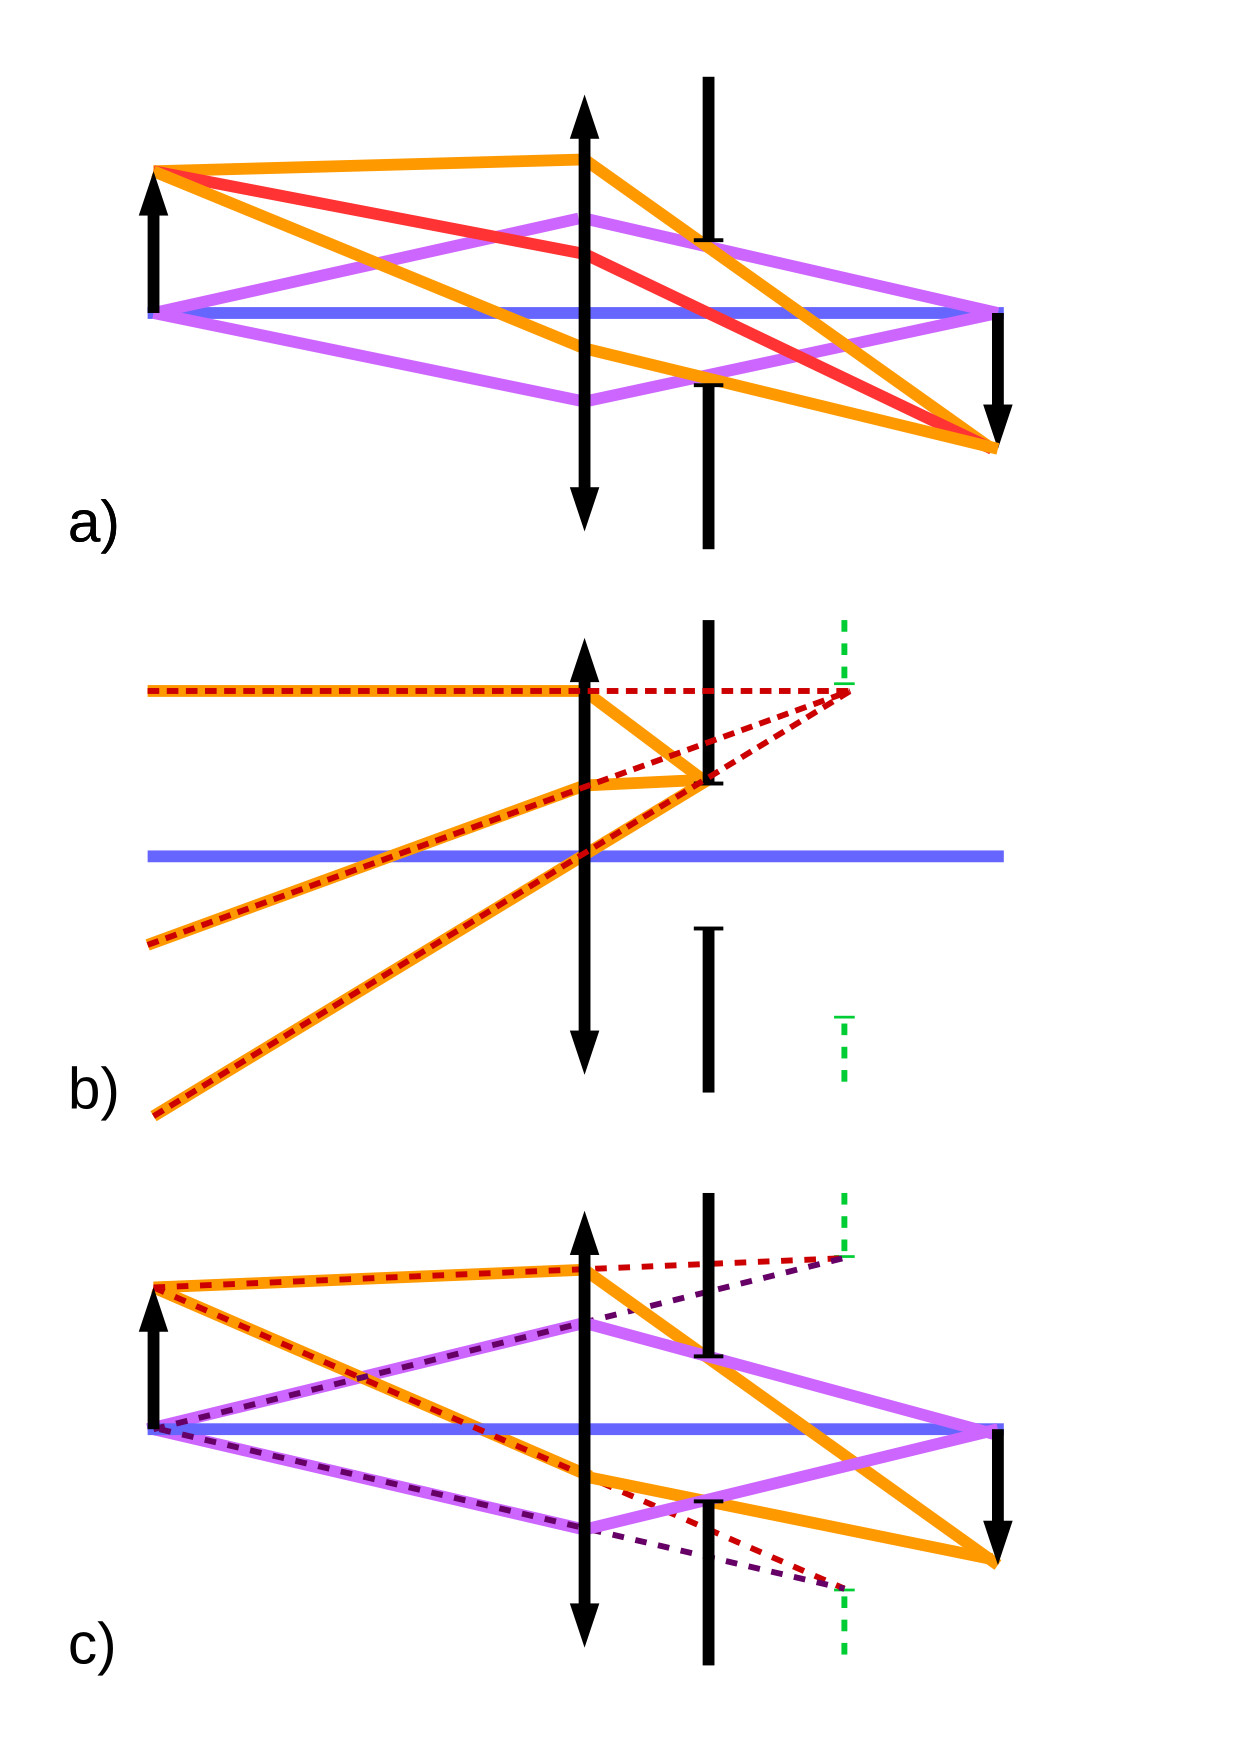
\includegraphics[width=0.5\columnwidth]{pupil}
  \caption{a) In an imaging system without vignetting, the stop acts as aperture for rays from all field points. The rays displayed are on-axis ray (blue), marginal rays (violet), chief ray (red), and coma rays (orange).
  b) In this system, the lens creates a virtual image of the stop, the pupil (green).
  c) The imaging relation between pupil and stop causes rays aimed at the pupil border to be refracted onto the stop border.
  }
  \label{fig:pupil}
\end{figure}


The optical system is capable of transmitting only a certain angular spectrum of the light emitted by each object field point.
We call the component which limits the amount of transmitted light for the on-axis field point \emph{stop}.
The stop can be, for example, the clear aperture of a finite sized lens or a metal ring aperture.
If at field points far from the axis also other elements start to clip rays, we call this additional clipping \emph{vignetting}.

The rays emitted by the central (on-axis) field point that hit the border of the stop are called \emph{marginal rays}.
The rays emitted by any non-zero field point that hit the border of the stop are called \emph{coma rays}.
The ray emitted by any non-zero field point that hits the center of the stop is called \emph{chief ray}.
Often, the chief ray is approximated to be the central ray in the ray bundle emitted by a field point.

We divide the optical systems into two groups -- elements in front of and behind the stop. 
We consider both groups of optical elements as systems imaging the stop.
We call the image of the stop created by the object sided elements \emph{entrance pupil}, and the image created by the image sided elements \emph{exit pupil}.

Rays in the object and rays in the entrance pupil need to pass the same group of optical elements in order to reach the stop. 
We can regard the propagation of rays from the object to the stop as a free space propagation from the object to the entrance pupil and a subsequent imaging into the stop.
In close analogy, we can image rays from the stop to the exit pupil and perform a free-space propagation from the exit pupil to the image.
This property is often used to determine the marginal and coma angles: 
aiming from the object into the entrance pupil by free-space propagation is much easier than tracing rays from the object to the stop.
Care has to be taken if the front lens group imaging the stop to the pupil suffers from aberrations such as distortion.


\section{Direction of the ray}
We assign a unit direction vector $\Vector{d}$ to each ray.
The direction vector points in the direction of the time averaged Poynting vector.
\begin{eqnarray}
 \Vector{d} &=& \frac{\timeavg{\Vector{S}}}{|\timeavg{\Vector{S}}|}
\end{eqnarray}

\section{Surface Normal}
Assume the surface of a material boundary is given in the form
\begin{eqnarray}
 z &=& z(x,y)
\end{eqnarray}
Two (infinitessimal) local in-plane vectors are 
\begin{eqnarray}
d\Vector{e}_1 = \begin{pmatrix}
                 dx \\ 0 \\ \frac{\partial z}{\partial x} dx
                \end{pmatrix}
\\
d\Vector{e}_2 = \begin{pmatrix}
                 0 \\ dy \\ \frac{\partial z}{\partial y} dy
                \end{pmatrix}
\end{eqnarray}
We normalize these local vectors and form the surface normal, perpendicular to both
\begin{eqnarray}
 \Vector{n} &=& \Vector{e}_1 \times \Vector{e}_2 \\
 &=& 
   \frac{1}{\sqrt{ 1 + \left( \frac{\partial z}{\partial x} \right)^2 + \left( \frac{\partial z}{\partial y} \right)^2 }}
   \begin{pmatrix}
    - \frac{\partial z}{\partial x} \\ - \frac{\partial z}{\partial y} \\ 1
   \end{pmatrix}
\end{eqnarray}

\section{Optical path length}
We define the optical path length as the time of travel of a near-monochromatic wavepacket times the vacuum speed of light.

In the special case of materials that can be described by an isotropic, real valued refractive index, the optical path length functional is given according to the Fermat principle,
\begin{align}
 L &= \int_{s_1}^{s_2} \underbrace{n(\Vector{r}(s)) |\Vector{r}'(s)|}_{=\mathcal{L}} \text{d}s\,.\label{eq:fermatiso}
\end{align}
with the corresponding ``Lagrangian'' $\mathcal{L}$.
$s$ is the arc length and therefore the derivative $\Vector{r}'(s)$ is a unit vector. (For the Euler Lagrange
equations we may not set it to $1$ at the moment.)

\remark{to do: all other cases; restriction to linear optics}


\section{Lagrange and Hamilton formalism}
Euler-Lagrange-Equations are given by
\begin{align}
 \frac{\text{d}}{\text{d}s} \frac{\partial \mathcal{L}}{\partial \Vector{r}'} &= \frac{\partial \mathcal{L}}{\partial \Vector{r}}\,.
\end{align}
The sloppy notation with vector derivatives means a differentiation by components.
\begin{align}
 \frac{\partial \mathcal{L}}{\partial \Vector{r}'} &= n(\Vector{r}(s)) \frac{\Vector{r}'(s)}{|\Vector{r}'(s)|} \stackrel{|\Vector{r}'(s)|=1}{=} n(\Vector{r}(s))\Vector{r}'(s)\,.
\end{align}
Therefore the appropriate differential equation (the so-called equation of motion, EOM) is given by
\begin{align}
 \frac{\text{d}}{\text{d}s} \left(n(\Vector{r}(s)) \frac{\text{d}\Vector{r}}{\text{d}s}\right) &= (\Vector{\nabla} n)(\Vector{r}(s)) \label{eq:ODEGRIN}\,.
\end{align}
( For a piecewise homogeneous medium the ODE system reduces to a system of algebraic equations 
[btw. this corresponds to a reduction of the
first variation of the integral to a first derivative of the corresponding sum].) 
For our later raytracing the initial conditions are given by:
\begin{subequations}
\label{eq:ODEGRINic}
\begin{align}
 \Vector{r}(s=0) &= (x,y,z)\,,\\
 \Vector{r}'(s=0) &= (d_x, d_y, \sqrt{1-d_x^2-d_y^2})\,,
\end{align}
\end{subequations}
where $\Vector{d}$ is the direction unit vector of some certain ray and $(x,y,z)$ is the starting position.
Now we may integrate \eqref{eq:ODEGRIN} for every set of initial conditions \eqref{eq:ODEGRINic}
and obtain after a (in general numerical) integration a set of values $\Vector{r}(s)$ and $\Vector{r}'(s)$
which correspond to the final position and direction of the ray.
\section{Hamiltonian Formulation}
There are two distinct parametrisations. The first one parametrizes the theory with respect to the
arc length $s$ in 3D space where (one possible choice of) the Hamiltonian is given by
\begin{align}
 H &= \Vector{p}^2 - n^2 = 0\,.
\end{align}
The canonical momentum $\Vector{p}$ is given by $\Vector{p} = n \Vector{d}$. (From this consideration the constraint on
the Hamiltonian becomes clear, since $|\Vector{d}| = 1$.) The canonical equations are given by
\begin{subequations}
\label{eq:H3Deom}
\begin{align}
 \frac{\text{d}\Vector{q}}{\text{d}s} &= \frac{\partial H}{\partial \Vector{p}} = 2 \Vector{p}\,,\\
 \frac{\text{d}\Vector{p}}{\text{d}s} &= -\frac{\partial H}{\partial \Vector{q}} = 2 n (\Vector{\nabla} n)\,, 
\end{align}
\end{subequations}
The second parametrisation is given by the $z$ position with respect to the optical axis. Here the Hamiltonian is
given by
\begin{align}
 H_{\text{2D}} &= -n(\Vector{Q}, z)\sqrt{1 - \frac{\Vector{P}^2}{n(\Vector{Q}, z)^2}}\label{eq:Hamiltonian2D}\,,
\end{align}
and is equal to the negative component of the 3D momentum.
This comes from the Legendre transformation of the Lagrangian
\begin{align}
 \mathcal{L} &= n(\Vector{Q}, z) \sqrt{1 + V^2}\,,
\end{align}
now parametrized by $z$ as independent variable, $\Vector{Q} = (x,y)$ and $\Vector{V} = (x'(z), y'(z))$.
The Legendre transformation involves first an inversion of the relation
\begin{align}
 \Vector{P} &= \frac{\partial \mathcal{L}}{\partial \Vector{V}} = n(\Vector{Q}, z) \frac{\Vector{V}}{\sqrt{1 + \Vector{V}^2}}\,,
\end{align}
with respect to $\Vector{V}$ and afterwards the calculation of
\begin{align}
 H_{\text{2D}}(\Vector{Q}, \Vector{P},z) &= \scpm{\Vector{P}}{\Vector{V}(\Vector{P})} - \mathcal{L}(\Vector{Q}, z, \Vector{P})\,,
\end{align}
which leads to \eqref{eq:Hamiltonian2D}. The equations of motion due to the canonical formalism 
are therefore given by [remember $\Vector{Q} = (x,y)$, $\Vector{P} = n (d_x, d_y)$]
\begin{subequations}
\label{eq:H2Deom}
\begin{align}
 \frac{\text{d}\Vector{Q}}{\text{d}z} &= \frac{\partial H_{\text{2D}}}{\partial \Vector{P}} = \frac{\Vector{P}}{n \sqrt{1 - \frac{\Vector{P}^2}{n^2}}}\,,\\
 \frac{\text{d}\Vector{P}}{\text{d}z} &= -\frac{\partial H_{\text{2D}}}{\partial \Vector{Q}} = \frac{\Vector{\nabla}_{\Vector{Q}} n}{\sqrt{1 - \frac{\Vector{P}^2}{n^2}}}\,.    
\end{align}
\end{subequations}
In general $n = n(\Vector{Q}, z)$ holds, so the Hamiltonian depends explicitly on the independent variable.
Therefore for $z$ dependent $n$ the Hamiltonian is no conserved quantity anymore and
\begin{align}
 \frac{\partial H_{\text{2D}}}{\partial z} &= -\frac{\frac{\partial n}{\partial z}}{\sqrt{1 - \frac{\Vector{P}^2}{n^2}}}\,.
\end{align}
(For constant $n$ this formulation is very similar to the Hamiltonian formulation of a 
massive particle in special relativity with imaginary linear momentum.
Therefore nearly all of the results there are applicable here. It is also very useful 
for the paraxial approximation which corresponds to a post-Newtonian expansion.)

\section{Numerical Integration for GRIN Media}
Let us start with the integration of the 3D formulation since it is separable $H = T + U$. Here we use a symplectic integration formalism
due to its symmetry preserving phase space integration structure. For the details we kindly refer the reader to the
literature. A symplectic integrator for a separable Hamiltonian is given by the following scheme with time step $h$:
\begin{align}
 \begin{pmatrix}
  \Vector{q} \\
  \Vector{p}
 \end{pmatrix} \mapsto
 \begin{pmatrix}
  \Vector{q} + c_i h \frac{\partial T}{\partial \Vector{p}} \\
  \Vector{p}
 \end{pmatrix}
\end{align}
and succesively
\begin{align}
 \begin{pmatrix}
  \Vector{q} \\
  \Vector{p}
 \end{pmatrix} \mapsto
 \begin{pmatrix}
  \Vector{q} \\
  \Vector{p} - d_i h \frac{\partial U}{\partial \Vector{q}}
 \end{pmatrix}\,.
\end{align}
For a fourth order scheme $i=1\dots4$ and the coefficients are given by
\begin{align}
 c_1 = c_4 = \frac{1}{2(2 - 2^{1/3})}\,,\\
 c_2 = c_3 = \frac{1 - 2^{1/3}}{2(2 - 2^{1/3})}\,,\\
 d_1 = d_3 = \frac{1}{2 - 2^{1/3}}\,,\\
 d_2 = -\frac{2^{1/3}}{2 - 2^{1/3}}\,\quad d_4 = 0\,.
\end{align}
For a further improvement it may be necessary to use adaptive ``time'' steps.
These can be implemented, e.g., by an extension of the phase space where
the time is an additional canonical coordinate. The extension is achieved by
a so-called Sundman transformation (which is in fact a Poincar{\'e} transformation)
of the ``time'' coordinate
$\text{d}s/\text{d}\sigma = g(\Vector{q}, \Vector{p})$.
By using a special form of this transformation $g$ the new Hamiltonian is separable and we
may use a symplectic scheme like the one mentioned above to integrate the new formulation.


\chapter{Raytracing}

Classical raytracing through stepwise homogeneous media consists of the following steps: 
The ray is considered a straight in 3D space. 
First its intersection point with the next surface is calculated geometrically. 
Then, a new wavevector is determined using the refraction law for plane waves on planar surfaces.

\section{Intersections of Straights with Spheres, Aspheres and Free-shapes}\label{subsec:intersectionformulas}

\subsection{Biconics}
A biconic describes a surface which has two perpendicular sections
which have a conic structure. These surfaces have two symmetry planes.
The explicit surface sag formula is given by
\begin{align}
 z &= \frac{\rho_x x^2 + \rho_y y^2}{1 + \sqrt{1 - (1+c_x) \rho_x^2 x^2 - (1+c_y) \rho_y^2 y^2}} \label{eq:biconic}\,.
\end{align}
The variables are $\rho_x = 1/R_x$ the $x$ curvature, $\rho_y = 1/R_y$ the $y$ curvature, $c_x$ the conic constant in $x$ direction,
and $c_y$ the conic constant in $y$ direction respectively. 

An invariant or implicit form of \eqref{eq:biconic} is given by
\begin{align}
 (a(x,y) - 1) z^2 + (z - b(x,y))^2 &= 0\,,\label{eq:implicitbiconic}
\end{align}
where $a(x,y) = (1 + c_x) \rho_x^2 x^2 + (1 + c_y) \rho_y^2 y^2$ and $b(x,y) = \rho_x x^2 + \rho_y y^2$. 
Inserting the ray straight equation \eqref{eq:ray}, this leads to a polynomial of fourth order.

\begin{eqnarray}
 \Location &=& \Location_0 + \Vector{d} t \label{eq:ray}
\end{eqnarray}
$\Location_0$ is the ray start point, $\Vector{d}$ the ray direction unit vector and $t$ the free parameter of the straight.

The fourth order equation can be solved either analytically or numerically.
Physically valid solutions must be real valued.


\subsection{Conics}
Conics are spheres, rotationally symmetric ellipsoids, paraboloids and hyperboloids.
The word ``conic" is short for conic section. This refers to these figures as the
intersections of a plane with a cone.
In the vertex form their surface sag $z$ can be described by
\begin{eqnarray}
 z =  \frac
 { \rho ( x^2 + y^2 ) }
 { 1 + \sqrt{1 - (1+c) \rho^2  (x^2 + y^2)} }\,,
\end{eqnarray}
where $c$ is the conic constant. Depending on this parameter, the conic is a
\begin{eqnarray*}
-1 < c < 0 && \textrm{oblate ellipsoid} \\
     c = 0 && \textrm{sphere} \\
 0 < c < 1 && \textrm{prolate ellipsoid} \\
     c = 1 && \textrm{paraboloid} \\
     c > 1 && \textrm{hyperboloid}
\end{eqnarray*}
For an explicit solution of the intersection parameter $t$,
one can use the implicit form of the surface equation
\begin{align}
 \rho (1 + c) z^2 - 2 z + \rho (x^2 + y^2) &=0\,.
\end{align}
After insertion of \eqref{eq:ray}, the solution is given by
\begin{subequations}
\label{eq:intersectionconicsection}
\begin{eqnarray}
   F &=& d_z - \rho \left( d_x x_0 + d_y y_0 + d_z z_0 (1+c) \right)\,, \\
   G &=& \rho (x_0^2 + y_0^2 + z_0^2 (1+c)) - 2 z_0\,, \\
   H &=& - \rho ( 1 + c \, d_z^2 )\,, \\
   t &=& \frac{G}{ F + \sqrt{F^2 + H G} }\,.
\end{eqnarray}
\end{subequations}

The unit surface normal of such a conic section pointing in forward (positive $z$) direction is
\begin{eqnarray}
\Vector{n} &=& - \frac{1}{\sqrt{ 1 - c (x^2 + y^2)}} 
  \begin{pmatrix}
   \rho x \\
   \rho y \\
   \rho ( 1 + c ) z - 1
  \end{pmatrix}
\end{eqnarray}




\subsection{Spheres}
\label{subsection:spheres}

We consider a ray and a Sphere that intersects the optical axis in the origin
\begin{eqnarray}
 \left| \Location - \begin{pmatrix} 0 \\ 0 \\ R \end{pmatrix} \right|^2 &=& R^2\,, \label{eq:sphereeq}
\end{eqnarray}
The standard manner to derive the solution would be to insert the ray equation \eqref{eq:ray} into
\eqref{eq:sphereeq} and calculate the solutions for $t$ from the arising quadratic equation. This leads to a numerically unstable solution
for large radii $R$.
A solution numerically stable for the case of a planar surface $R \rightarrow \infty$ is:
\begin{subequations}
\label{eq:spheresolution}
\begin{eqnarray}
   F &=& d_z - \rho \scpm{\Vector{d}}{\Location_0}\,, \\
   G &=& \rho |\Location_0|^2 - 2 z_0\,, \\
   H &=& - \rho\,, \\
   t &=& \frac{G}{ F + \sqrt{F^2 + H G} }\,, \label{eq:tsolsphere}
\end{eqnarray}
\end{subequations}
where $\rho = 1 / R$ is the surface curvature. 
The solution exists for positive terms under the square root only, $F^2 + H G > 0$. 
Otherwise, the ray misses the sphere.

The unit surface normal of the sphere pointing in forward (positive $z$) direction is
\begin{eqnarray}
\Vector{n} &=& -  
  \begin{pmatrix}
   \rho x \\
   \rho y \\
   \rho z - 1
  \end{pmatrix}
\end{eqnarray}


\subsection{Conical Acylinder}
A conical acylinder is the special case $\rho_x=0, c_x=0$ of a biconic. It contains cylindric and simple acylindric lenses like elliptical, parabolic and hyperbolic acylindric lenses.
Without loss of generality, we choose our coordinate system so that the curvature in x-direction vanishes.
This effectively reduces the problem of an intersection in three-dimensional space to a two-dimensional one.

\begin{align}
 z &= \frac{ \rho y^2}{1 + \sqrt{1 - (1+c) \rho^2 y^2}}
\end{align}
The solution is
\begin{eqnarray}
   F &=& d_z - \rho \left(  d_y y_0 + d_z z_0 (1+c) \right) \\
   G &=& \rho ( y_0^2 + z_0^2 (1+c)) - 2 z_0 \\
   H &=& - \rho ( 1 + c \, d_z^2 ) \\
   t &=& \frac{G}{ F + \sqrt{F^2 + H G} }
\end{eqnarray}


\subsection{Cylindric}
A cylindric surface is the special case $c = 0$ of a conical acylinder.
\begin{align}
 z &= \frac{ \rho y^2}{1 + \sqrt{1 - \rho^2 y^2}}
\end{align}
The solution further simplifies to
\begin{eqnarray}
   F &=& d_z - \rho \left(  d_y y_0 + d_z z_0  \right) \\
   G &=& \rho ( y_0^2 + z_0^2 ) - 2 z_0 \\
   H &=& - \rho \\
   t &=& \frac{G}{ F + \sqrt{F^2 + H G} }
\end{eqnarray}


\subsection{Polynomial Asphere}

For a polynomial asphere the general form is
\begin{align}
  z &=  \frac
 { \rho ( x^2 + y^2 ) }
 { 1 + \sqrt{1 - (1+c) \rho^2  (x^2 + y^2)} } + A(x^2 + y^2)\,,
\end{align}
where $A$ is a polynomial starting at second order in the given variable.
The appropriate equation to find the intersection point is given by [completing the square and so on]\remark{check!}
\begin{align}
 \left(z - A(x^2 + y^2) - \frac{1}{\rho(1+c)}\right)^2 - \frac{1}{\rho^2 (1+c)^2} \left(1 -(1+c)\rho^2 (x^2 + y^2) \right) &= 0\,.
\end{align}
The first term is strictly positve, the second is always negative if the ray should hit the asphere. For the calculation
of the intersection point one has to insert the ray parameters for $x, y, z$ and calculate the intersection parameter $t$.
In the present case this is only possible numerically. 


\subsection{Strong Forbes Asphere}
to do
\subsection{Mild Forbes Asphere}
to do
\subsection{Acylindric}
to do

\subsection{Free Shapes}
to do

\subsection{Linear Combinations}
\remark{I would suggest to implement a few standard forms and to combine them by a linear combination operator. This makes the search for optimizable
variables more difficult.}



\section{Ray Aiming}
The caculation of many aberrations requires tracing a fan of rays or a ray bundle rastering the whole pupil.
Often, the desired size of the pupil is not given explicitly, but the optical designer wants to specify a f-number or a numerical aperture.
This section deals with the conversion between different pupil and field descriptions and how to find suitable starting positions and directions of rays in the object plane.
If possible, we prefer a description that is numerically stable for telecentric systems and infinite conjugate systems.

\subsection{Ray origin for finite conjugate objects}
For finite conjugate objects, the object plane is part of the optical system. Rays from one field point originate from the same point in the object plane.

to do

\subsection{Ray origin for infinite conjugate objects}
to do

\subsection{Ray directions}
We want to cast rays from the ray origin positions so that they hit certain coordinates in the pupil plane. 
The na\"{\i}ve ansatz to subtract the ray origin from the desired pupil coordinate to obtain the ray direction will likely fail numerically for telecentric systems.
Therefrore, we derive the marginal ray slope and the chief ray slope from the first order properties of the system and base the ray directions on these two quantities.
%
\begin{eqnarray}
  \left. \frac{\partial x}{\partial z}\right|_{ray} &=& \left. \frac{\partial x}{\partial z}\right|_{chief} + \left. \frac{\partial x}{\partial z}\right|_{marginal} \cdot x_{pup} \\
  \left. \frac{\partial y}{\partial z}\right|_{ray} &=& \left. \frac{\partial y}{\partial z}\right|_{chief} + \left. \frac{\partial y}{\partial z}\right|_{marginal} \cdot y_{pup}
\end{eqnarray}
where $x_{pup}, y_{pup} \in [-1,1]$ are pupil coordinates normalized to the pupil radius. 
An equidistant mesh of pupil coordinates will may result in a constant ray density per solid angle, especially for high-NA systems or systems with large field angles.
A non-equidistant sampling grid limits the validity of fast-Fourier based calculation methods.

\subsubsection{Paraxial pupil aiming}
In paraxial pupil aiming, the optical system is represented by ABCD-Matrices and the marginal slope is calculated paraxially.
We split the optical system into one ABCD Matrix from the object to the stop
\begin{eqnarray*}
 ABCD_{obj\rightarrow stop} &=&
 \begin{pmatrix}
  A_o & B_o \\ C_o & D_o
 \end{pmatrix}
\end{eqnarray*}
and one matrix from the stop to the image
\begin{eqnarray*}
 ABCD_{stop\rightarrow ima} &=&
 \begin{pmatrix}
  A_i & B_i \\ C_i & D_i
 \end{pmatrix}
\end{eqnarray*}
The pupil is the image of the stop, imaged by the front lens group $ABCD_{obj\rightarrow stop}$ for the entrance pupil and the rear lens group $ABCD_{stop\rightarrow ima}$ for the exit pupil, respectively.
The entrance pupil is imaged to distance $z_{en}$ from the object and appears to be magnified in size by a factor of $mag_{en}$ compared to the stop. 
Similarly, the exit pupil has a distance $z_{ex}$ from the image and a magnification of $mag_{ex}$.
\begin{eqnarray}
 z_{en} &=& \frac{B_o}{A_o} \\
 mag_{en} &=& \frac{1}{A_o} \\
 z_{ex} &=& - \frac{B_i}{D_i} \\
 mag_{ex} &=& A_i - \frac{B_i C_i}{D_i}
\end{eqnarray}
For telecentric systems, an expression of the pupil rastering in terms of $z_{en}$ or $z_{ex}$ is depreceated. 
Expressing everything in terms of ABCD matrices, it is often possible to reduce fractions analytically and avoid numerical instabilities.

\section{Wave Aberrations}
Despite its name suggests this representation of aberrations would be based on wave optics, its calculation is purely geometrical.
Wave aberrations are strongly related to the optical path difference.

\subsection{Optical path difference}
In a perfect lens (made of isotropic, lossless materials), all rays from one object point to an image point have the same optical path length, according to the law of Fermat. 
In systems with aberrations, the optical path length from object to image is different for rays passing different pupil positions.

The optical path difference $OPD$ is the optical path length minus the optical path length of the chief ray.
\begin{eqnarray}
 OPD(p_x,p_y) &=& L(p_x,p_y) - L(0,0)
\end{eqnarray}
For a certain fixed object field point, the optical path difference is often displayed as a function of pupil coordinates $p_x,p_y$.

For anisotropic or lossy materials, the Fermat law no longer holds, and a finite optical path difference from object to image is no more synonomous to aberrations.
In this case, the interpretation becomes more complex.

\subsection{Wave Aberrations}
To obtain the so called wave aberration, one first calculates the optical path difference from an object point to the image plane.
Then, a reference surface is constructed. 
Each point of the reference surface shall have the same optical path length to the chief ray image point.
For isotropic media, the reference surface becomes a sphere.
The radius of the sphere is chosen so that the surface intersects the optical axis at the exit pupil position, together with the chief ray.

All rays are then propagated backwards from the image to the reference surface.
The back-propagation is performed with the dispersion of the last material before the image, 
for example the image sided immersion liquid or the glass of a field lens glued onto the detector.
If there is an air gap between last lens and detector, the air dispersion is to be used.
In many cases, the back-propagation length is larger than the backfocal length of the system.

The wave aberrations are the optical path differences from object to exit pupil, 
that is the optical difference from object to image minus the path difference of the back-propagation.
By definition, the wave aberration of the chief ray is zero.
Typically, wave aberrations are displayed as a map over the two-dimensional exit pupil coordinates.
For imaging systems, the wave aberrations relative to the chief ray are typically very small, and are often displayed in units of vacuum wavelengths.

Using the Huygens principle, the field in the exit pupil can be interpreted as a set of point sources, radiating in the image direction. 
They form an Eikonal wavefront identical to that of the rays traced from object to image.
In technical optics, at this point often wave and ray optics are intermixed:
From the exit pupil to the image, a Huygens propagation is performed numerically exact in wave optics, resulting in a spot that cannot surpass the diffraction limit. 
The retardation of each point-source, however, is calculated using geometrical optics.
In a system without any aberrations made of isotropic materials, all point-sources are in phase and form a spherical wave segment, converging towards a spot of minimal spatial extent.
All aberrations cause a perturbation of the spherical wave, and an extended spot size.
The accurracy of the result compared to full physical wave-optical calculations of the point-spread function of the whole system is often astonishing. 

To reduce calculation times, the electric field map of the emitters in the curved exit pupil is often assumed planar and equidistant. 
The normalized ray coordinates in entrance and exit pupil are assumed to be identical.
A rectangular raster in the entrance pupil will thus result in a rectangular raster in the exit pupil.
Exit pupil and image are assumed Fourier-conjugate, allowing the use of fast Fourier methods.
The tremendous gain in speed is often worth the sacrifice in accuracy in optimisation tasks to get close to a diffraction limited system.
In the final optimisation step, it may be worth using the more accurate Huygens propagation method.

\begin{figure}
  \centering
   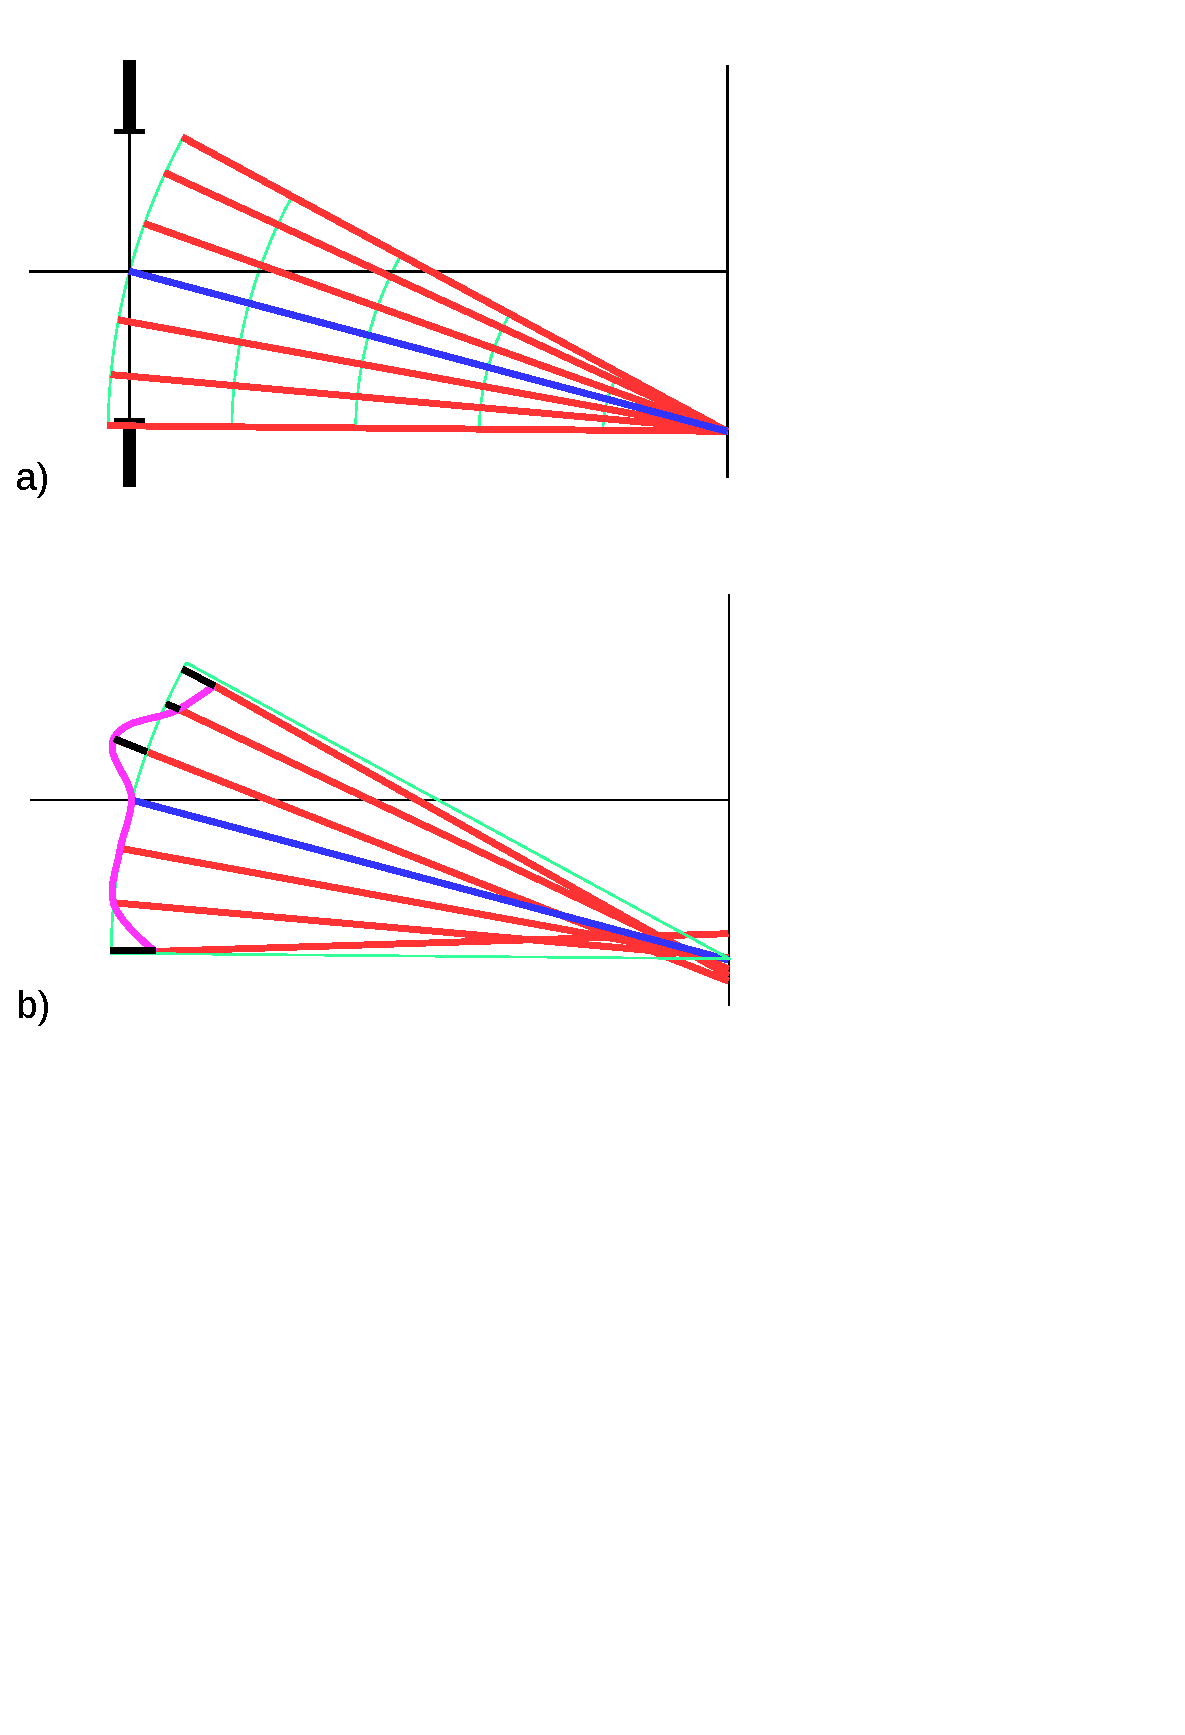
\includegraphics[width=0.5\columnwidth]{waveaberrations}
  \caption{a) In a perfect system, according to the Fermat principle, all rays have the same time of flight from the object to the image. b) In a real system, wave aberrations occur. A line of constant time of flight is displayed in magenta.
  Wave aberrations are the optical path differences corresponding to the difference in time of flight when hitting the exit pupil reference sphere.}
  \label{fig:waveaberrations}
\end{figure}

\subsection{Calculation of wave aberrations}
\remark{this only works for on axis field points}

Assume we know the position $x_{im}, y_{im}$ and direction $\Vector{d}$ of a set of rays in the image plane and their geometric path length from the object to the image.
To obtain the wave aberrations, we intersect the rays with the spherical exit pupil.
The task is similar to the intersections performed throughout the raytracing, see section \ref{subsection:spheres}.
We center our coordinate system around the chief ray image position.

\begin{eqnarray}
 \Location &=& \begin{pmatrix} x_0 \\ y_0 \\ 0 \end{pmatrix} + \Vector{d} t \\
 \Location^2 &=& R^2
\end{eqnarray}
with
 \begin{eqnarray}
 \begin{pmatrix} x_0 \\ y_0 \end{pmatrix} &=& \begin{pmatrix} x_{im} \\ y_{im} \end{pmatrix} - \begin{pmatrix} x_{chief,im} \\ y_{chief,im} \end{pmatrix} \\
 z_{im} &=& 0 \\
 | \Vector{d} | &=& 1
\end{eqnarray}
Here, $R$ is the distance between exit pupil and image, and $t$ is the geometric path length of the back-propagation.

We find
\begin{eqnarray}
 R^2 &=&  t^2 + 2 (d_x x_0 + d_y y_0) t + x_0^2 + y_0^2 \\
 t_{1,2} &=& - (d_x x_0 + d_y y_0) \pm \sqrt{ (d_x x_0 + d_y y_0)^2 - (x_0^2 + y_0^2) + R^2 }
\end{eqnarray}

We assume that the macroscopic distance between image and exit pupil $R^2$ term under the root is much larger than the microscopic aberrations and use a Taylor expansion
\begin{eqnarray}
 t_{1,2} &\approx& R - (d_x x_0 + d_y y_0) \pm 
 \left[ 
   \frac{1}{2R} \delta - \frac{1}{8R^3} \delta^2
 \right]
 \\
 \delta &=& (d_x x_0 + d_y y_0)^2 - x_0^2 - y_0^2
\end{eqnarray}

The geometric path length $t$ is inserted into the material dispersion to obtain the retardation between exit pupil and image. After that, this propagation length is subtracted from the optical path length from object to image.
Another subtraction of the chief ray value normalizes the result.
By didviding with the vacuum wavelength, we obtain the wave aberration in number of waves.



\end{document}
